\documentclass[9.5pt,a4paper]{article}
\usepackage[utf8]{inputenc}
\usepackage[spanish,es-tabla]{babel}
\usepackage[top=1.2cm,bottom=1.2cm,left=1.4cm,right=1.4cm]{geometry}
\usepackage{microtype}
\usepackage{xcolor}
\usepackage{titlesec}
\usepackage{enumitem}
\usepackage{tcolorbox}
\usepackage{url}
\usepackage{hyperref}
\usepackage{booktabs}
\usepackage{tabularx}
\usepackage{fancyhdr}
\usepackage{array}
\usepackage{graphicx}

% Ajuste de interlineado y listas compacto
\setlength{\parindent}{0pt}
\setlength{\parskip}{2.5pt}
\setlist{noitemsep, topsep=1pt, parsep=0pt, partopsep=0pt, leftmargin=*}

% Paleta de colores ejecutiva
\definecolor{primary}{RGB}{27, 54, 93}      % Azul Marino Institucional (#1B365D)
\definecolor{secondary}{RGB}{46, 134, 171}  % Azul Acero (#2E86AB)
\definecolor{accent}{RGB}{224, 90, 71}      % Coral (#E05A47)
\definecolor{teal}{RGB}{0, 168, 150}        % Verde Azulado (#00A896)
\definecolor{lightgray}{RGB}{248, 249, 250} % Fondo suave (#F8F9FA)
\definecolor{bordercolor}{RGB}{220, 225, 230}% Borde de cajas

\hypersetup{
    breaklinks=true,
    colorlinks=true,
    linkcolor=primary,
    filecolor=secondary,      
    urlcolor=secondary,
    citecolor=accent
}

% Formato compacto de títulos
\titleformat{\section}
  {\color{primary}\normalfont\normalsize\bfseries}{\thesection.}{0.4em}{}[\titlerule]
\titleformat{\subsection}
  {\color{secondary}\normalfont\small\bfseries}{\thesubsection.}{0.3em}{}

\titlespacing*{\section}{0pt}{4pt}{1.5pt}
\titlespacing*{\subsection}{0pt}{2.5pt}{1pt}

% Encabezados y pie de página
\pagestyle{fancy}
\fancyhf{}
\fancyhead[L]{\footnotesize\textcolor{gray}{Visualización 1 -- Proyecto 2: Análisis Reproducible en Python (WHR 2024)}}
\fancyhead[R]{\footnotesize\textcolor{gray}{Documento Ejecutivo y Metodológico}}
\fancyfoot[C]{\footnotesize Página \thepage\ de 4}
\renewcommand{\headrulewidth}{0.3pt}

% Cajas compactas
\tcbset{
    colback=lightgray,
    colframe=primary,
    arc=1.2mm,
    boxrule=0.6pt,
    left=6pt,
    right=6pt,
    top=3pt,
    bottom=3pt
}

\begin{document}

% =========================================================================
% PÁGINA 1: AUDIENCIA, PREGUNTA ANALÍTICA Y PREPARACIÓN DE DATOS
% =========================================================================
\begin{center}
    {\scriptsize\textbf{\color{secondary}UNIVERSIDAD EXTERNADO DE COLOMBIA \quad|\quad FACULTAD DE FINANZAS, GOBIERNO Y RR.II.}}\\[0.03cm]
    {\large\textbf{\color{primary}Proyecto 2: Visualización Reproducible en Python (Seaborn \& Plotly)}}\\[0.03cm]
    {\normalsize\textbf{Informe Técnico-Ejecutivo: Arquitectura y Determinantes del Bienestar Global (WHR 2024)}}\\[0.1cm]
    \rule{\linewidth}{0.6pt}\\[0.05cm]
    \footnotesize
    \begin{tabularx}{\linewidth}{@{}X X@{}}
        \textbf{Fuente Oficial:} World Happiness Report 2024 (\texttt{Figure 2.1.xls}) & \textbf{Investigadores:} Julián Duarte y Julián Jiménez \\
        \textbf{Fecha de Entrega:} Octubre de 2026 & \textbf{Docentes:} Adriana Pineda Barón y Paola Moreno
    \end{tabularx}\\[0.02cm]
    \rule{\linewidth}{0.6pt}
\end{center}

\vspace{-0.15cm}

\section{Audiencia Técnica Específica y Contexto Estratégico}
El informe está dirigido a la \textbf{Comisión Técnica de Evaluación de Políticas de Bienestar de Organismos Multilaterales de Cooperación y Desarrollo (ej. PNUD / OCDE / BID)}. Esta unidad técnica reúne a investigadores cuantitativos y economistas del desarrollo responsables de:
\begin{itemize}
    \item \textbf{Focalización de recursos:} Priorizar asistencia técnica en regiones vulnerables sujetas a trampas estructurales de bajo bienestar.
    \item \textbf{Evaluación multidimensional:} Superar la visión unidimensional del PIB, analizando el rol del capital social, la libertad cívica y la probidad gubernamental.
    \item \textbf{Reproducibilidad y rigor:} Auditar un flujo de trabajo enteramente verificable en código abierto, con transformaciones y decisiones metodológicas transparentes.
\end{itemize}

\section{Problemática y Formulación de la Pregunta Analítica}
Históricamente, los planes internacionales asumieron que el crecimiento del ingreso per cápita traducía automáticamente en bienestar subjetivo. Sin embargo, regiones de renta media como América Latina exhiben niveles de bienestar superiores a lo proyectado económicamente, mientras naciones con alto ingreso sufren estancamientos. Ante este reto empírico, formulamos la siguiente pregunta:

\begin{tcolorbox}[colback=primary!5!white, colframe=primary, title=\textbf{\color{white}\small Pregunta Analítica Central}]
\centering\small
\textit{¿Cómo se diferencian los perfiles de bienestar entre las macro-regiones del mundo y en qué medida los factores relacionales e institucionales (soporte social, libertad individual y percepción de corrupción) explican la resiliencia en países de ingreso medio frente a aquellos estancados en trampas de bajo bienestar subjetivo?}
\end{tcolorbox}

\section{Auditoría de Datos, Variables y Protocolo de Preparación}
Se procesó el conjunto oficial \texttt{WHR24\_Data\_Figure\_2.1.xls} ($N = 143$ países, $11$ variables cuantitativas):
\begin{enumerate}
    \item \textbf{Auditoría de Integridad y Nulos:} Únicamente 3 países presentan valores ausentes en las variables explicadas (\textit{Bahrain}, \textit{Tajikistan} y \textit{State of Palestine}), manteniéndose para distribuciones generales y aislándose sin sesgo en modelos explicativos.
    \item \textbf{Mapeo Regional Oficial (ONU / WHR):} Se clasificaron los 143 países en las 10 macro-regiones oficiales (cobertura $100\%$).
    \item \textbf{Variables Clave:} Evaluación de vida (\texttt{Ladder score}), Riqueza (\texttt{Log GDP}), Soporte Social (\texttt{Social support}), Esperanza de vida saludable (\texttt{Healthy life expectancy}), Libertad individual (\texttt{Freedom}), Transparencia (\texttt{Corruption}) y \texttt{Generosity}.
\end{enumerate}

\vspace{0.05cm}
\begin{center}
\footnotesize
\renewcommand{\arraystretch}{1.08}
\begin{tabularx}{\linewidth}{@{}p{3.8cm} c c c p{4.5cm}@{}}
\toprule
\textbf{Macro-Región WHR 2024} & \textbf{Países ($N$)} & \textbf{Mediana} & \textbf{Desv. Est.} & \textbf{Patrón Observado en Bienestar} \\ \midrule
\textbf{Norteamérica y ANZ} & 4 & 6.93 & 0.14 & Liderazgo de alta homogeneidad global. \\
\textbf{Europa Occidental} & 20 & 6.84 & 0.54 & Alto bienestar con elevada equidad distributiva. \\
\textbf{Europa Central y Oriental} & 17 & 6.30 & 0.44 & Convergencia acelerada hacia el bloque occidental. \\
\textbf{América Latina y Caribe} & 19 & 6.14 & 0.43 & Resiliencia social y dividendo relacional frente al PIB. \\
\textbf{Asia Oriental} & 6 & 5.75 & 0.44 & Alta renta con rezago relativo en soporte subjetivo. \\
\textbf{Comunidad Estados Indep.} & 10 & 5.56 & 0.55 & Dispersión moderada en economías de transición. \\
\textbf{Sudeste Asiático} & 9 & 5.37 & 0.81 & Marcada polarización interna (Singapur vs. Camboya). \\
\textbf{Medio Oriente y N. África} & 16 & 5.16 & 1.25 & Máxima heterogeneidad y volatilidad institucional. \\
\textbf{África Subsahariana} & 35 & 4.38 & 0.70 & Rezago estructural y trampas de vulnerabilidad. \\
\textbf{Asia del Sur} & 6 & 4.14 & 0.94 & Región más vulnerable del planeta (Afganistán: 1.72). \\ \bottomrule
\end{tabularx}
\end{center}

\clearpage

% =========================================================================
% PÁGINA 2: EVIDENCIA CON SEABORN (CUATRO VISUALIZACIONES ESTÁTICAS)
% =========================================================================
\section{Análisis Exploratorio: Patrones, Relaciones y Brechas con Seaborn}

Desarrollamos cuatro visualizaciones estáticas fundamentadas en principios de percepción visual (Gestalt, alto data-to-ink ratio):

\vspace{-0.1cm}
\begin{center}
    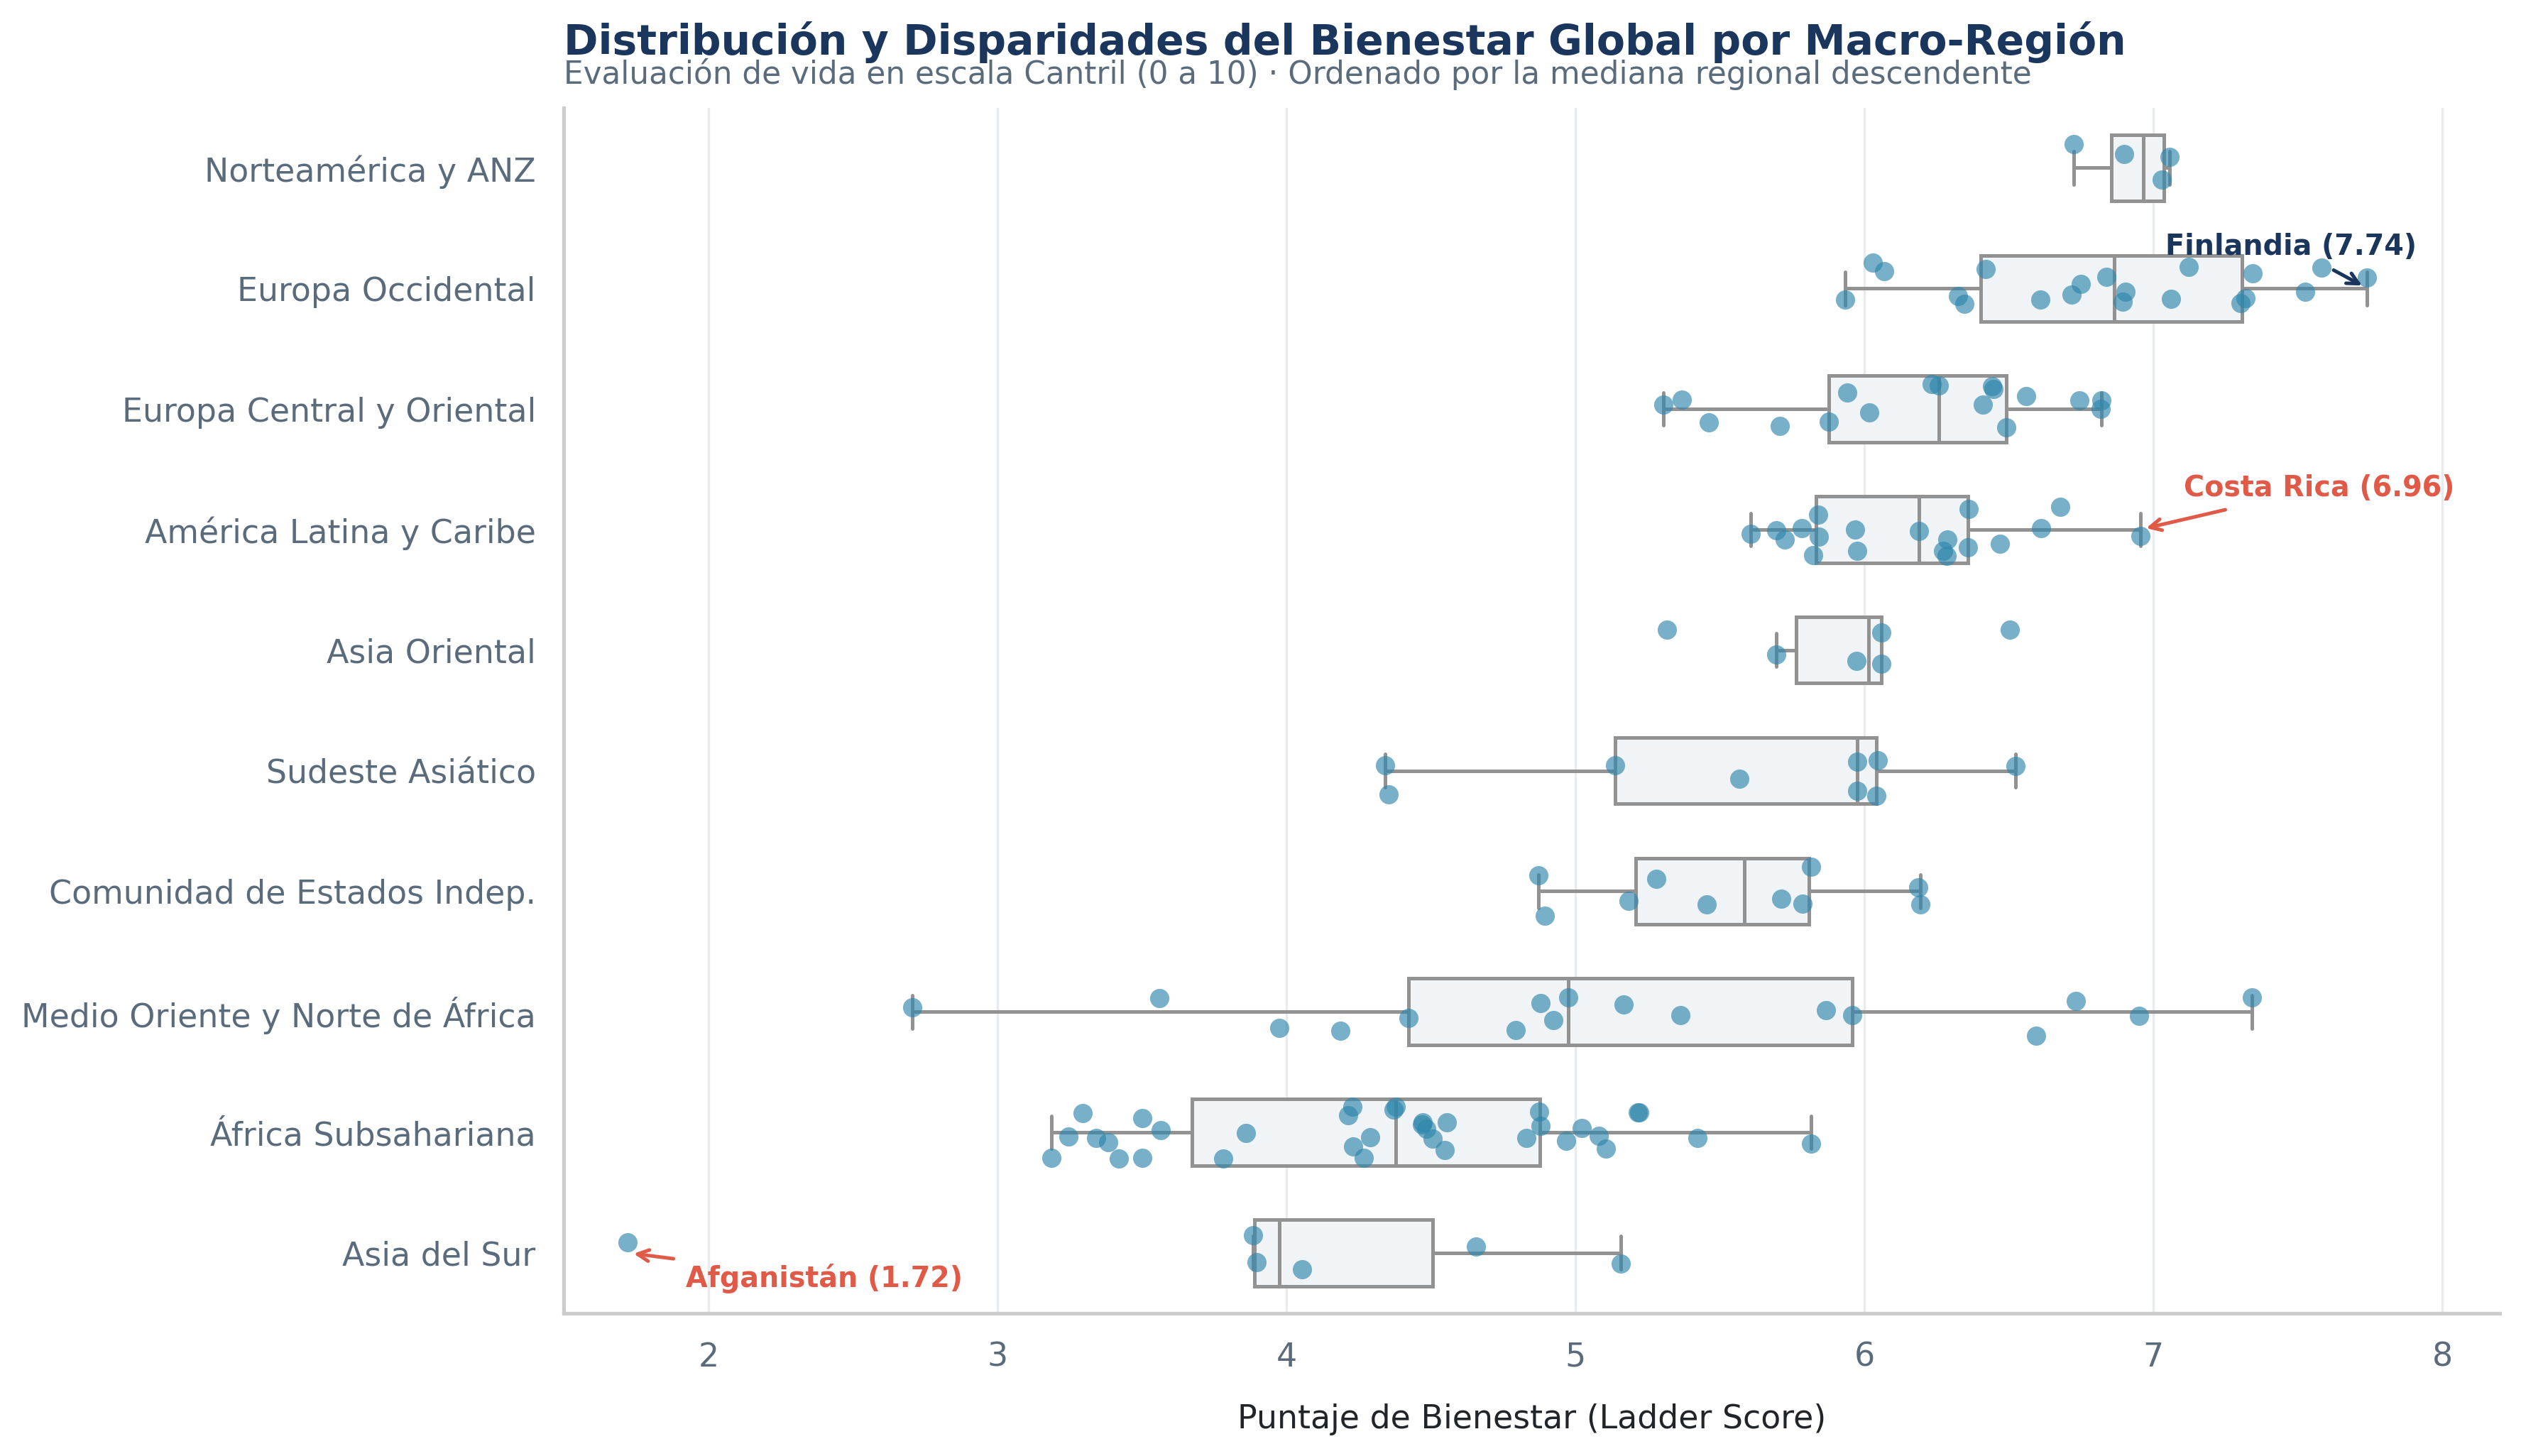
\includegraphics[width=0.92\linewidth, height=4.2cm, keepaspectratio]{figuras/fig1_distribucion_regional.png}
\end{center}
\vspace{-0.3cm}
\textbf{Interpretación 1 (Distribución Regional):} El bienestar exhibe una fractura bipolar: \textit{Norteamérica y ANZ} (mediana: $6.93$) y \textit{Europa Occidental} ($6.84$) lideran con distribuciones compactas en la cúspide. En contraste, \textit{Medio Oriente y Norte de África} registra una dispersión extrema ($\sigma = 1.25$, desde Israel y EAU hasta Yemen y Líbano). \textit{América Latina y el Caribe} (mediana: $6.14$) supera el promedio global, superando a regiones de mayor ingreso per cápita como Asia Oriental ($5.75$).

\vspace{0.1cm}
\begin{minipage}[t]{0.48\linewidth}
    \centering
    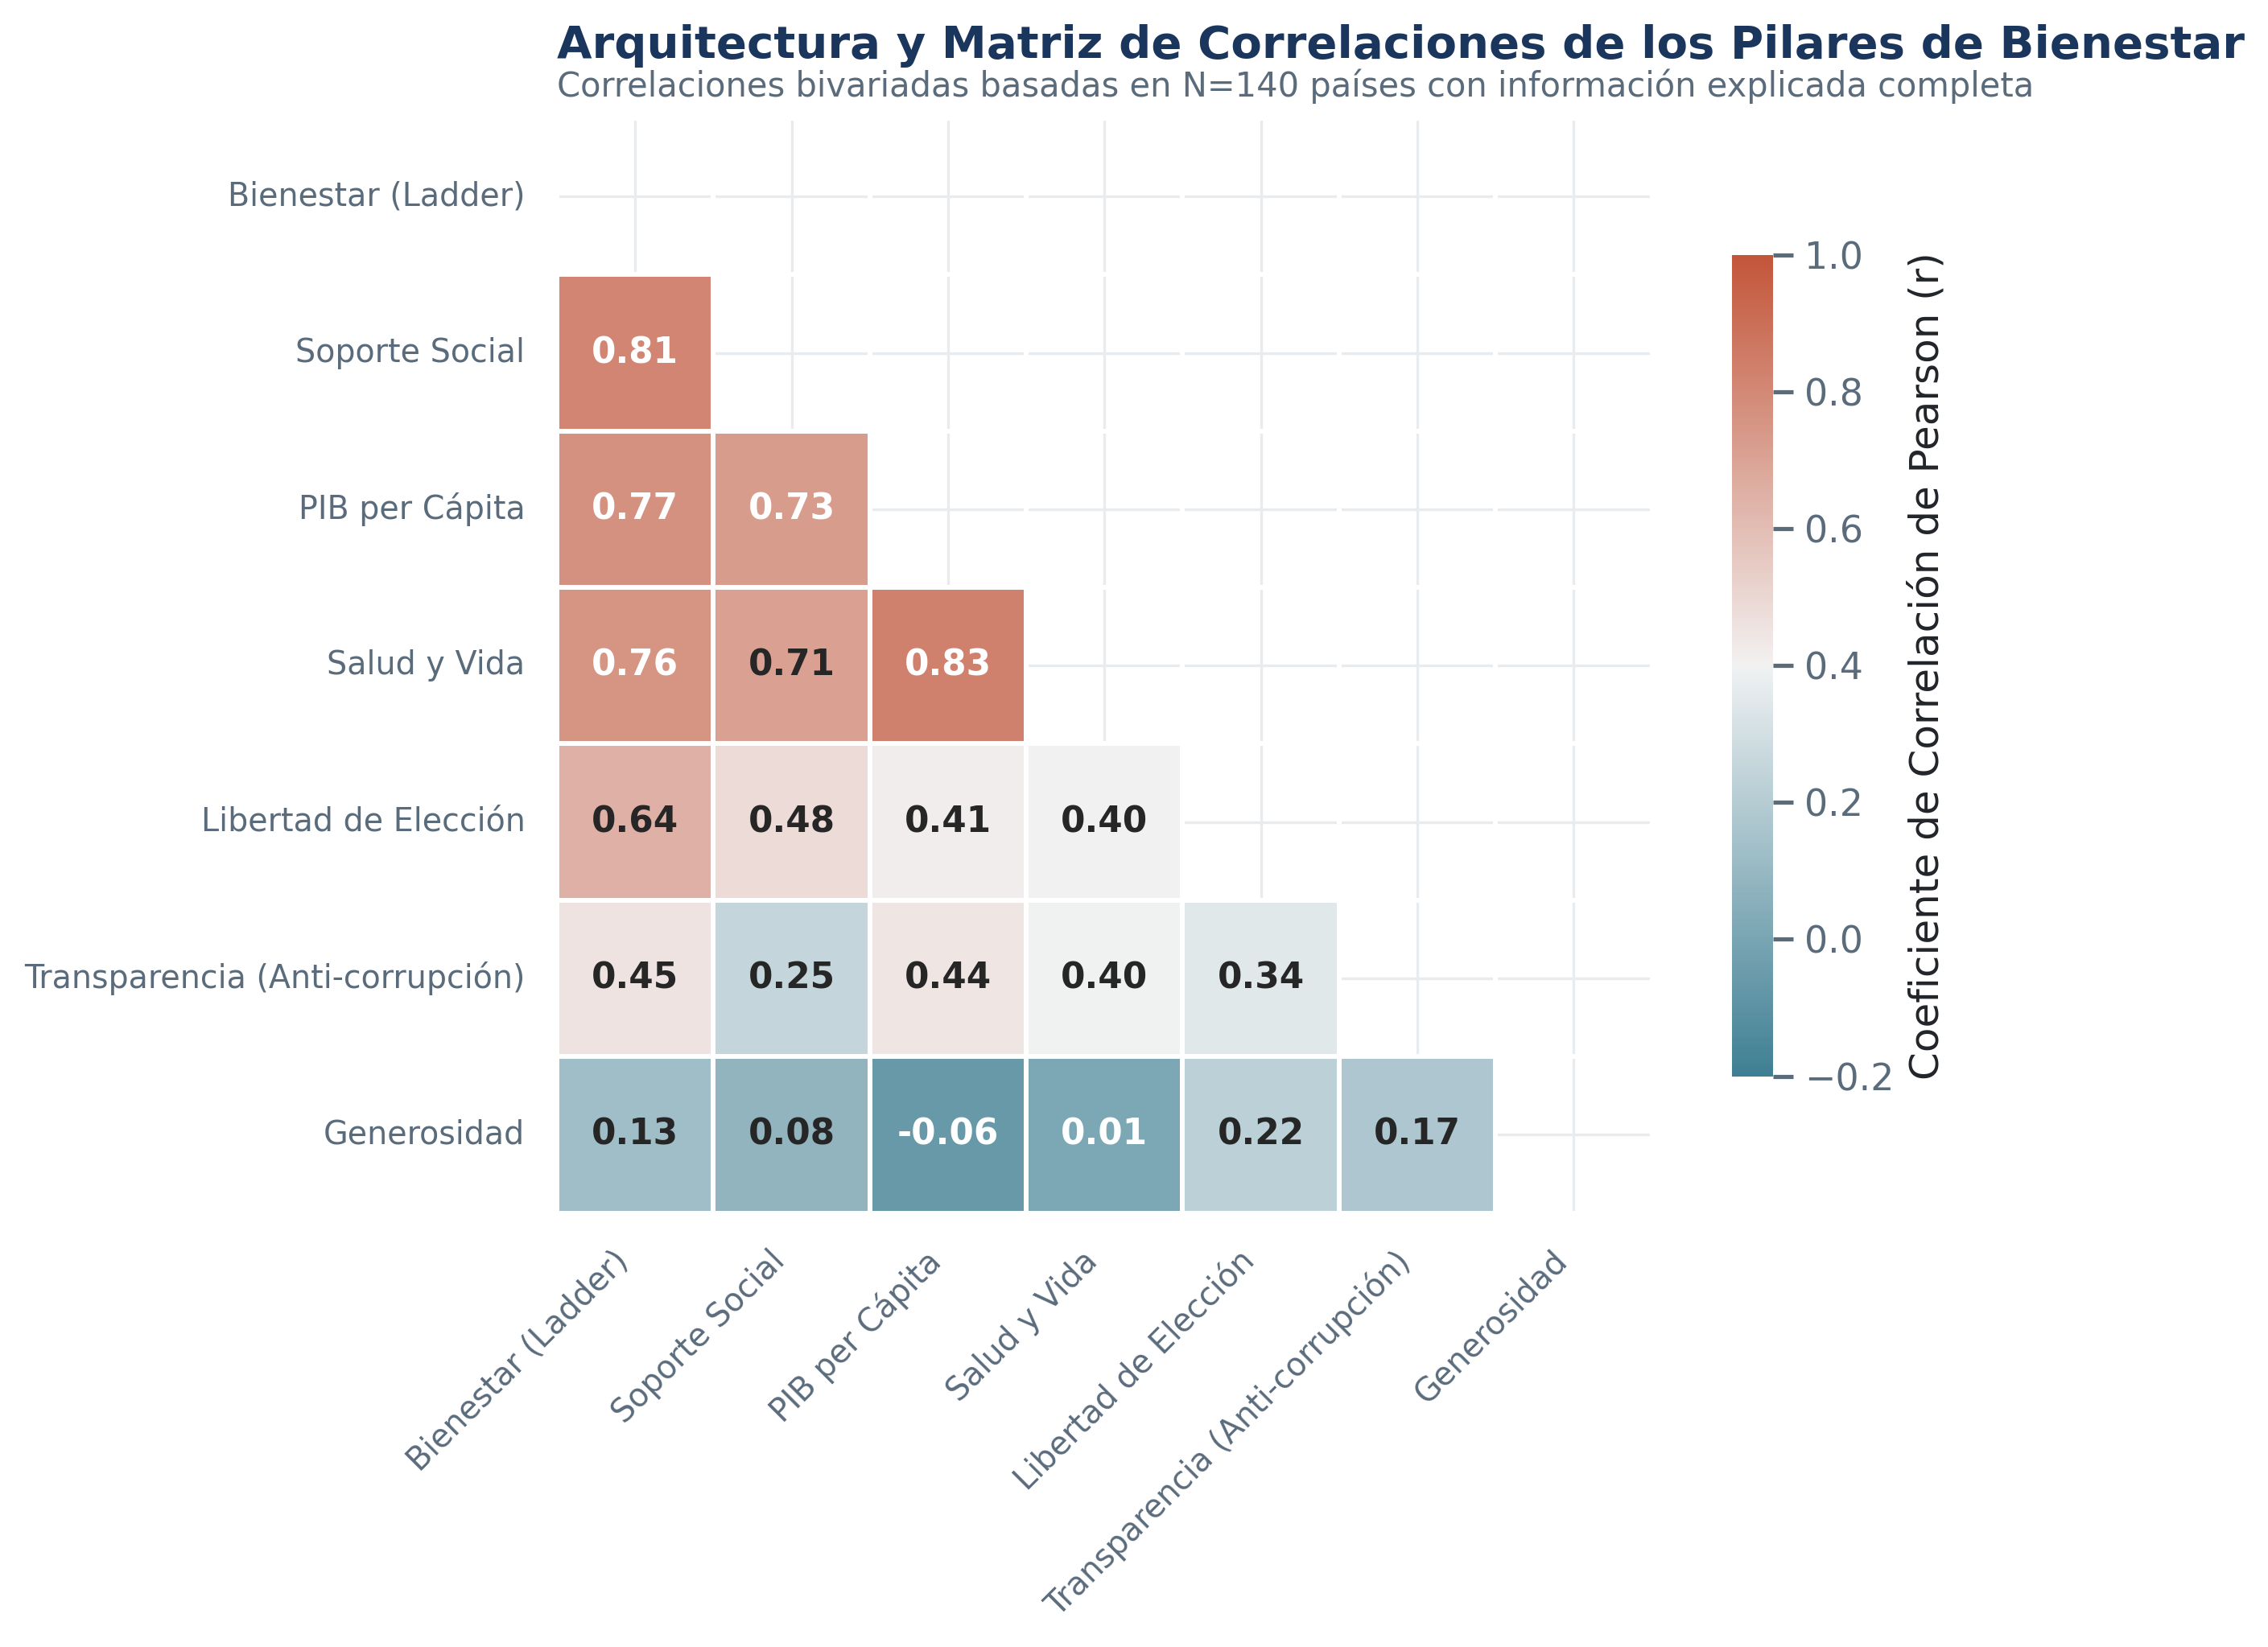
\includegraphics[width=\linewidth, height=4.1cm, keepaspectratio]{figuras/fig2_matriz_correlaciones.png}\\[-0.15cm]
    {\footnotesize\textbf{Interpretación 2 (Matriz de Correlaciones):} El factor con mayor correlación individual con el bienestar general es el \textbf{Soporte Social} ($r = 0.81$), superando al PIB per cápita ($r = 0.77$) y a la salud ($r = 0.76$). El tejido relacional humano es la base primaria del bienestar colectivo.}
\end{minipage}
\hfill
\begin{minipage}[t]{0.48\linewidth}
    \centering
    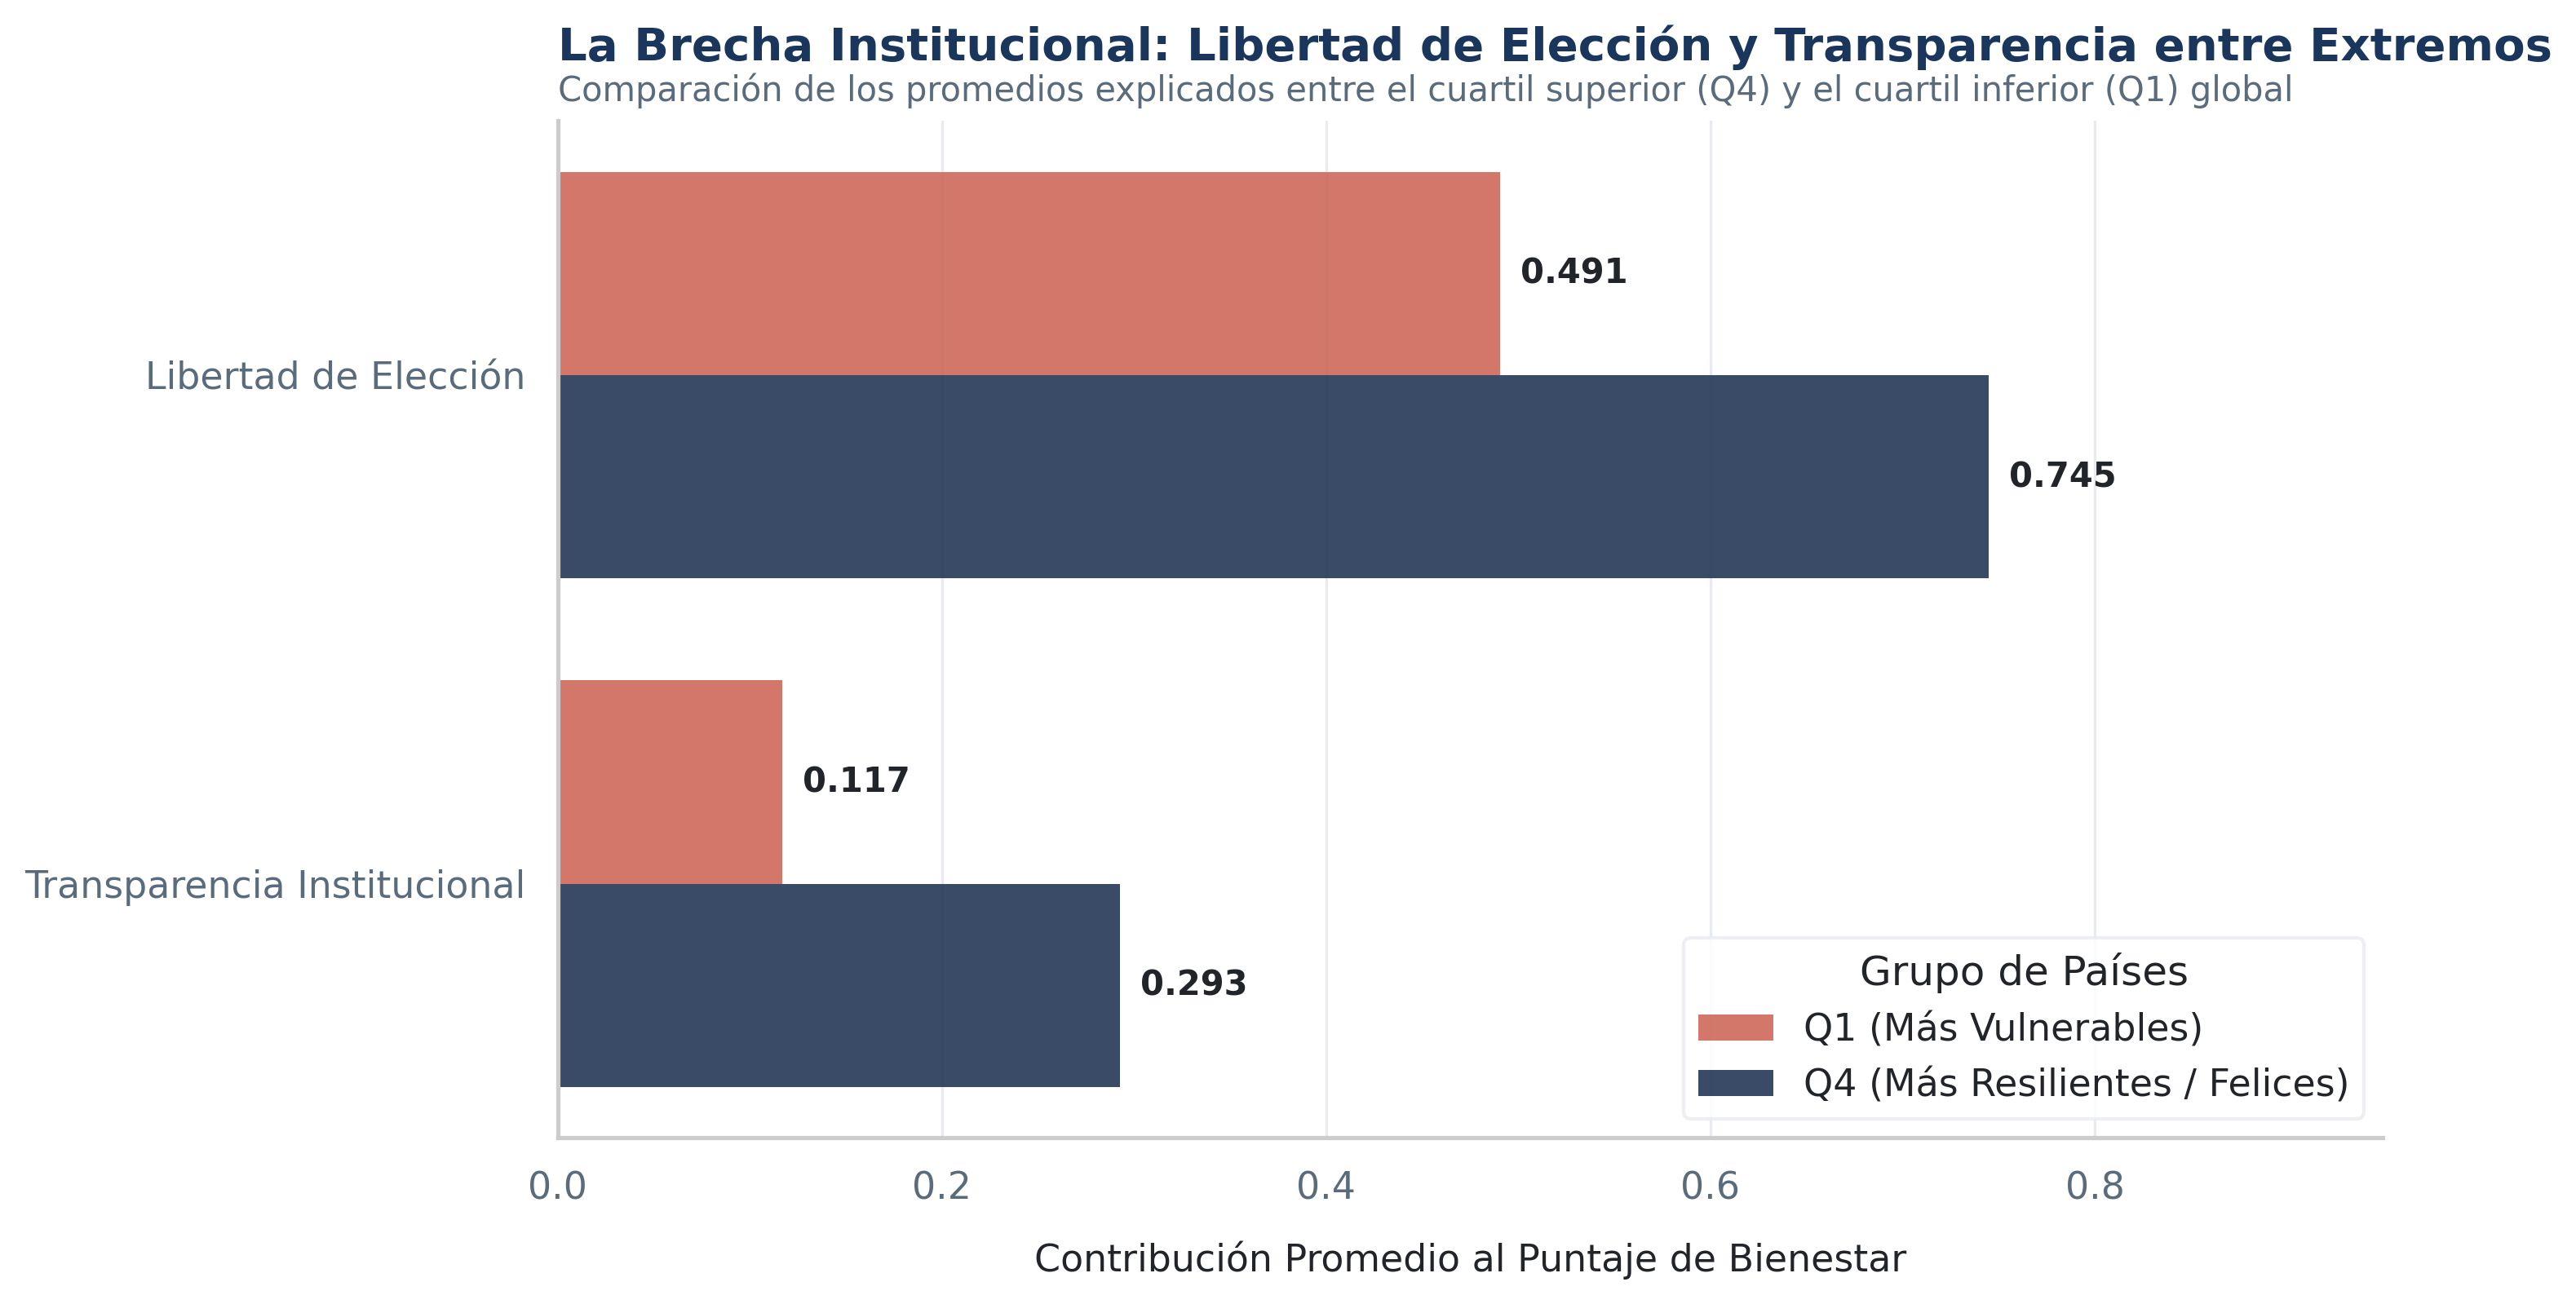
\includegraphics[width=\linewidth, height=4.1cm, keepaspectratio]{figuras/fig4_brecha_institucional.png}\\[-0.15cm]
    {\footnotesize\textbf{Interpretación 4 (Brechas Institucionales Q4 vs Q1):} En el cuartil más resiliente ($Q4$), el aporte de la transparencia gubernamental es \textbf{3.7 veces superior} ($0.279$ vs. $0.076$ en $Q1$) y la libertad individual es $62\%$ mayor ($0.730$ vs. $0.449$). La corrupción actúa como un techo estructural asfixiante.}
\end{minipage}

\vspace{0.15cm}
\begin{center}
    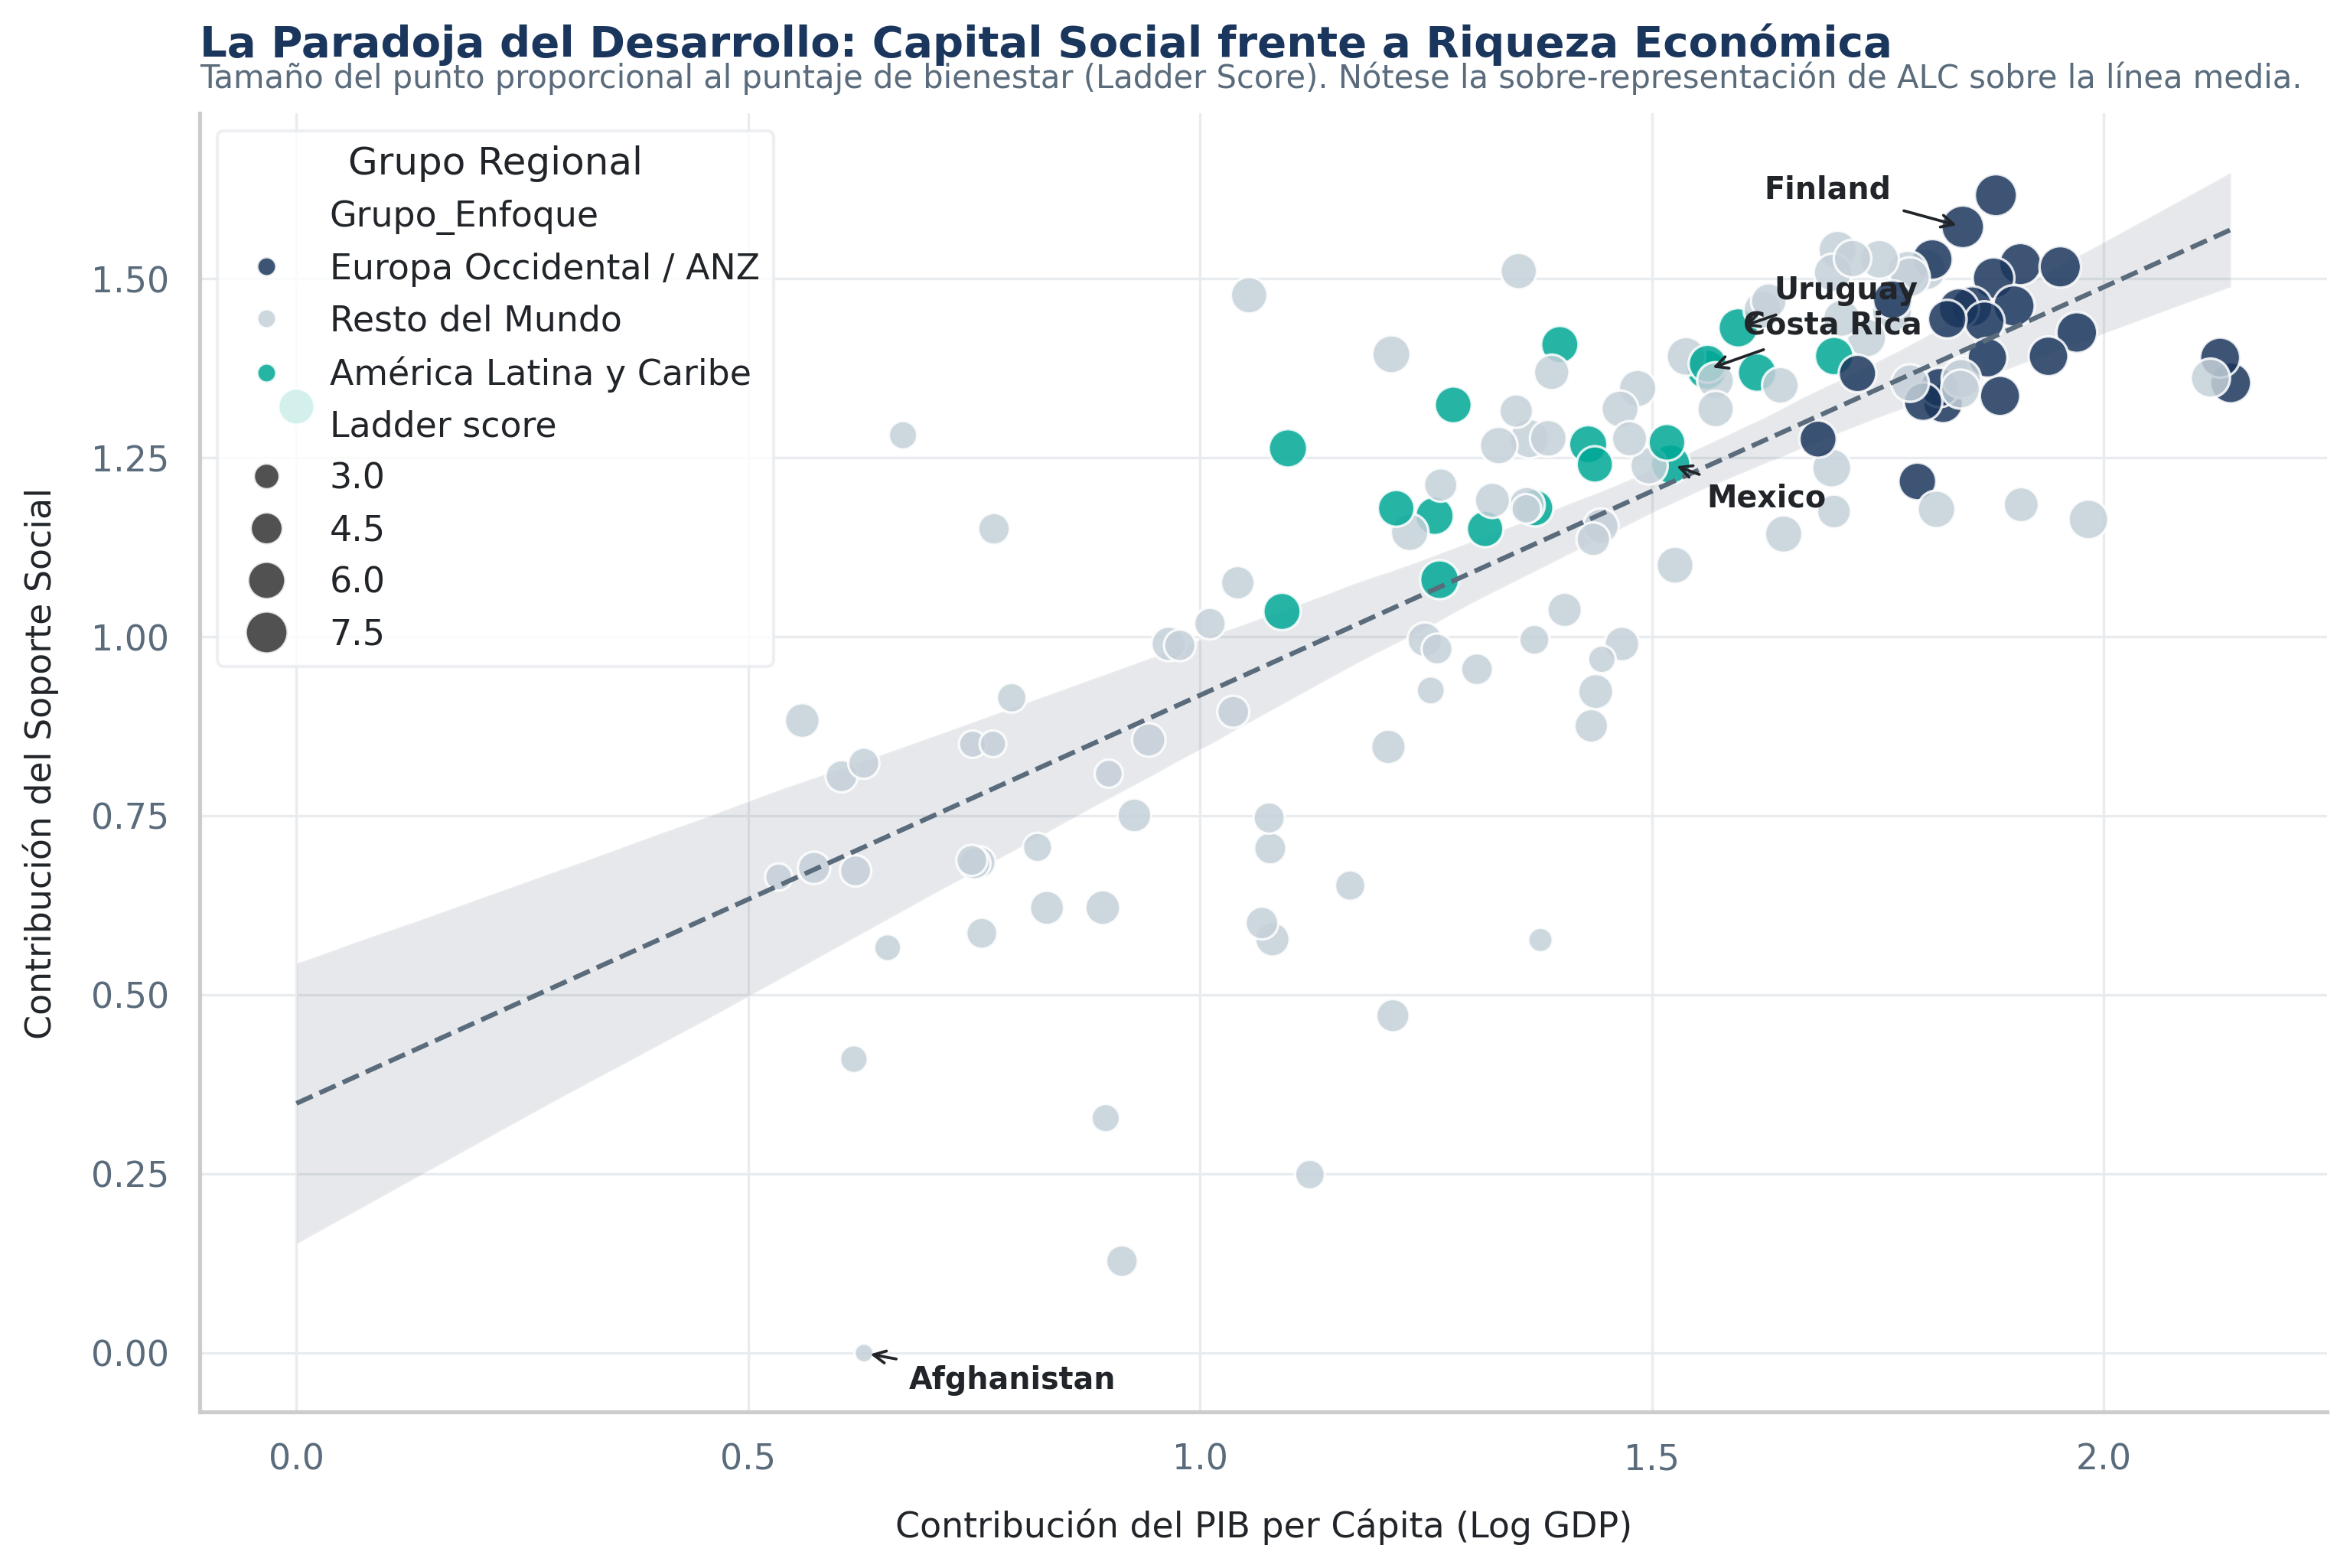
\includegraphics[width=0.92\linewidth, height=4.2cm, keepaspectratio]{figuras/fig3_paradoja_desarrollo.png}
\end{center}
\vspace{-0.3cm}
\textbf{Interpretación 3 (La Paradoja del Desarrollo y el Dividendo Relacional):} La regresión lineal OLS demuestra que los países de América Latina y el Caribe (puntos turquesa) se ubican sistemáticamente \textbf{por encima de la línea de ajuste global}. Países como Costa Rica, El Salvador, Uruguay, México y Colombia consolidan un soporte social equiparable al de Europa Occidental disponiendo de una fracción de su renta económica.

\clearpage

% =========================================================================
% PÁGINA 3: INTERACTIVIDAD EN PLOTLY, SÍNTESIS Y POLÍTICA PÚBLICA
% =========================================================================
\section{Exploración Interactiva en Plotly y Valor Analítico Agregado}
El archivo entregable autocontenido (\texttt{Equipo\_Duarte\_Jimenez\_Proyecto2\_Visualizaciones\_Interactivas.html}) incorpora dos tableros interactivos para auditar en vivo la evidencia empírica:
\begin{enumerate}
    \item \textbf{Explorador Multidimensional de Bienestar:} Integra 4 dimensiones simultáneas: PIB per cápita (Eje X), Longevidad Saludable (Eje Y), Soporte Social (tamaño de burbuja) y Macro-región (color). Permite aislar regiones en la leyenda y realizar inspección puntual por país mediante tooltips detallados.
    \item \textbf{Descomposición Dinámica de Factores (Stacked Bars):} Incorpora un menú selector dinámico (\texttt{updatemenus}) para comparar los 6 componentes explicativos aditivos de la felicidad junto al residuo de distopía para el Top 15, Bottom 15 y las 10 macro-regiones de la ONU.
\end{enumerate}

\section{Conclusiones Estratégicas y Respuesta a la Pregunta Analítica}
\begin{enumerate}[label=\textbf{C\arabic*.}]
    \item \textbf{El PIB es condición necesaria pero insuficiente:} El crecimiento económico garantiza solvencia material básica, pero sus rendimientos marginales sobre la felicidad se aplanan rápidamente. Las naciones más felices combinan riqueza con redes de soporte y libertades civiles.
    \item \textbf{El Capital Social como amortiguador de vulnerabilidad:} El soporte social ($r = 0.81$) ejerce un rol protector decisivo en economías en desarrollo. La evidencia latinoamericana demuestra que la cohesión familiar y cívica atenúa el impacto de la desigualdad económica.
    \item \textbf{La trampa de corrupción e institucionalidad débil:} La asfixia institucional por corrupción (diferencia de casi 4 veces entre extremos) impide a los países del cuartil inferior traducir inversión en bienestar ciudadano.
\end{enumerate}

\section{Recomendaciones de Acción para Organismos Multilaterales}
\begin{tcolorbox}[colback=lightgray, colframe=primary, title=\textbf{\color{white}\small Recomendaciones para la Junta Directiva de Cooperación}]
\begin{enumerate}[label=\textbf{R\arabic*.}]
    \item \textbf{Reorientar condicionalidades de préstamos de ayuda:} Incorporar metas explícitas de preservación comunitaria y capital social, superando la exclusividad en metas cuantitativas de crecimiento del PIB.
    \item \textbf{Priorizar inversión en transparencia activa y gobierno abierto:} La erradicación de la corrupción ofrece el mayor retorno marginal por dólar invertido en calidad de vida ciudadana en naciones vulnerables.
    \item \textbf{Fortalecer espacios de autonomía cívica:} Blindar la libertad individual de toma de decisiones frente a políticas asistencialistas paternalistas que limitan la autogestión comunitaria.
\end{enumerate}
\end{tcolorbox}

\subsection*{Limitaciones Metodológicas y Cautela Inferencial}
Los datos reflejan un corte transversal trianual promedio (2021--2023). Por tanto, \textbf{las correlaciones observadas no deben interpretarse como relaciones causales mecánicas}. Igualmente, la escala Cantril puede contener variaciones culturales de respuesta asociadas a normas sociales de optimismo o reserva.

\clearpage

% =========================================================================
% PÁGINA 4: ANEXO TÉCNICO DE USO DE IA (MÁXIMO 1 PÁGINA)
% =========================================================================
\section{Anexo Técnico de Uso de Herramientas de Inteligencia Artificial}

En concordancia con los principios de transparencia y ética académica de la Universidad Externado de Colombia, se declara el uso asistencial de modelos de lenguaje durante el desarrollo del proyecto:

\subsection*{1. Herramientas Utilizadas y Propósito General}
\begin{itemize}
    \item \textbf{Herramienta:} Google Gemini (Asistente de Programación y Visualización Antigravity AI).
    \item \textbf{Propósitos:} Asistencia en la depuración y estandarización del código en Python (Seaborn y Plotly), calibración de paletas cromáticas accesibles e institucionalización de la maquetación tipográfica en \LaTeX.
\end{itemize}

\subsection*{2. Registro de Prompts Clave Empleados}

\begin{tcolorbox}[colback=lightgray, colframe=bordercolor, title=\textbf{\small Prompt 1: Paleta Cromática y Accesibilidad Visual}]
\footnotesize
\textit{"Diseña una paleta cromática sobria e institucional de alto contraste para un informe de bienestar ante una junta directiva de la OCDE/PNUD. Proporciona códigos HEX diferenciados para variables continuas, categorías y advertencias (ej. Azul Marino \#1B365D, Azul Acero \#2E86AB, Coral \#E05A47, Verde Azulado \#00A896). Asegura que el contraste sobre fondo blanco cumpla normas WCAG y no dependa exclusivamente del color para comunicar jerarquías."}
\end{tcolorbox}

\begin{tcolorbox}[colback=lightgray, colframe=bordercolor, title=\textbf{\small Prompt 2: Cautela Inferencial y Narrativa Analítica}]
\footnotesize
\textit{"Estructura la interpretación analítica de los gráficos de correlación entre PIB y bienestar subjetivo en el WHR 2024. El tono debe ser el de un equipo de científicos de datos dirigiéndose a una junta directiva de desarrollo internacional: riguroso, evitando categóricamente presentar correlación como causalidad, y enfatizando el rol amortiguador del soporte social."}
\end{tcolorbox}

\begin{tcolorbox}[colback=lightgray, colframe=bordercolor, title=\textbf{\small Prompt 3: Solución de Compatibilidad en Seaborn 0.13 y Pandas 3.0}]
\footnotesize
\textit{"Al filtrar cuartiles Q1 y Q4 de una variable categórica generada con pd.qcut, Seaborn 0.13 arroja un ValueError por claves faltantes en el diccionario de paleta. ¿Cómo se ajusta de forma limpia y reproducible sin alterar el tipado de los datos originales?"}
\end{tcolorbox}

\subsection*{3. Reflexión Crítica, Auditoría y Validación Humana}
El equipo integrado por \textbf{Julián Duarte} y \textbf{Julián Jiménez} auditó y validó de forma crítica todas las respuestas y sugerencias del modelo:
\begin{itemize}
    \item \textbf{Verificación Empírica y Cero Alucinación:} Todos los coeficientes ($r = 0.81$, brechas de $3.7\times$, medianas regionales) fueron calculados directamente ejecutando el código sobre el archivo oficial \texttt{WHR24\_Data\_Figure\_2.1.xls}.
    \item \textbf{Auditoría de Código y Reproducibilidad:} Las soluciones propuestas para la generación del HTML interactivo y las exportaciones gráficas fueron probadas de inicio a fin en el entorno de desarrollo, asegurando que el Notebook se ejecute limpiamente.
    \item \textbf{Criterio Humano de Autoría:} Las decisiones analíticas sobre la audiencia técnica, el diseño de la pregunta de investigación y las conclusiones estratégicas corresponden al criterio exclusivo de los investigadores.
\end{itemize}

\vspace{0.2cm}
\begin{tcolorbox}[colback=lightgray, colframe=primary, title=\textbf{\color{white}\small Repositorio y Recursos Entregables}]
\footnotesize
\textbf{Acceso al Repositorio de Código:} Todos los recursos reproducibles (Jupyter Notebook, datos oficiales, figuras en alta resolución y archivo HTML interactivo) se encuentran organizados y archivados en el repositorio oficial de GitHub del proyecto.
\end{tcolorbox}

\end{document}
